\documentclass[11pt,dvipsnames,usenames,aspectratio=169]{beamer}  % Add handout to options to disable overlays

% For more themes, color themes and font themes, see:
% http://deic.uab.es/~iblanes/beamer_gallery/index_by_theme.html
%
\mode<presentation>
{%
  \usetheme{CambridgeUS}    % or try default, Darmstadt, Warsaw, ...
  \usecolortheme{whale}     % or try albatross, beaver, crane, ...
  \usefonttheme{serif}          % or try default, structurebold, ...
  % \usefonttheme[onlymath]{serif}
  % \setbeamertemplate{navigation symbols}{}
  % \setbeamercovered{transparent}

  \setbeamercolor{title}{fg=white}
  \setbeamerfont{title}{series=\bfseries}
  \setbeamercolor{frametitle}{fg=black}
  \setbeamerfont{frametitle}{series=\bfseries}

  \setbeamercolor{section in head/foot}{fg=white}
  \setbeamerfont{section in head/foot}{series=\bfseries}
  \setbeamercolor{subsection in head/foot}{fg=white}
  \setbeamerfont{subsection in head/foot}{series=\bfseries}
  \setbeamercolor{author in head/foot}{fg=white}
  \setbeamerfont{author in head/foot}{series=\bfseries}
  \setbeamercolor{title in head/foot}{fg=white}
  \setbeamerfont{title in head/foot}{series=\bfseries}

  \setbeamercolor{block title}{use=structure,fg=white,bg=title in head/foot.bg}
  \setbeamerfont{block title}{series=\bfseries}
  \setbeamercolor{block body}{use=structure,fg=black,bg=black!1!white}
}

% Support graying out frame elements
\newcommand{\FrameOpague}{\setbeamercovered{again covered={\opaqueness<1->{40}}}}
% Transition slide
\newcommand{\transitionFrame}[1]{%
{%
  \begin{frame}[plain,noframenumbering]{}{} % the plain option removes the sidebar and header from the title page
    \setbeamertemplate{final page}[text]{\Large \textbf{#1}}
    \usebeamertemplate{final page}
  \end{frame}}
}

% \usepackage{hyperref}     % Loaded automatically by beamer
\usepackage{pgfplots}       % Used to generate embedded plots
\pgfplotsset{compat=1.13}

% Here's where the presentation starts, with the info for the title slide
\title[Towards Deep Robustness]{Towards Deep Learning Models \\ Resistant to Adversarial Attacks\texorpdfstring{~\cite{Madry:2017}}{}}
\author[\madry]{%
  \href{mailto:madry@mit.edu}{Aleksander Madry}\inst{1}  % \textsuperscript{(\Letter)}
  \and
  \href{mailto:amakelov@mit.edu}{Aleksandar Makelov}\inst{1}  % \textsuperscript{(\Letter)}
  \and
  \href{mailto:ludwigs@mit.edu}{Ludwig Schmidt}\inst{1}  % \textsuperscript{(\Letter)}
  \and
  \href{mailto:tsipras@mit.edu}{Dimitris Tsipras}\inst{1}  % \textsuperscript{(\Letter)}
  \and
  \href{mailto:avladu@mit.edu}{Adrian Vladu}\inst{1}  % \textsuperscript{(\Letter)}
  % \href{mailto:lowd@cs.uoregon.edu}{Daniel Lowd}\inst{1}
}

\institute[MIT]{%
  \textsuperscript{1}\textbf{MIT -- CSAIL}\\
  % \texttt{{zayd, lowd}@ucsc.edu}
}
\date{\today}

\newcommand{\etal}{et~al.}
\newcommand{\elkan}{Elkan \&~Noto}

% Used for including standalone docs
\usepackage{standalone}

% Imported via UltiSnips
% Unbreakable dash:
%  Words hyphened with these dashes can also be broken at other positions than the dash
%    \-/ hyphen
%    \-- en-dash
%    \--- em-dash
%    extdash unbreakable dashes
%
%  No line breaks possible at the hyphen
%    \=/ hyphen
%    \== en-dash
%    \=== em-dash
\usepackage[shortcuts]{extdash}

% Imported via UltiSnips
\usepackage{color}
\newcommand{\colortext}[2]{{\color{#1} #2}}
\newcommand{\red}[1]{\colortext{red}{#1}}
\newcommand{\blue}[1]{\colortext{red}{#1}}
\newcommand{\green}[1]{\colortext{green}{#1}}

% Imported via UltiSnips
\usepackage{amsmath}
\DeclareMathOperator*{\argmax}{arg\,max}
\DeclareMathOperator*{\argmin}{arg\,min}
\DeclareMathOperator{\sgn}{sgn}
\usepackage{amsfonts}  % Used for \mathbb and \mathcal
\usepackage{amssymb}

% Imported via UltiSnips
\usepackage{mathtools} % for "\DeclarePairedDelimiter" macro
% \swapifbranches changes unstarred paired delimiters to starred and
% vice versa.  This means by default, paired delimiters have the star.
\usepackage{etoolbox}
\newcommand\swapifbranches[3]{#1{#3}{#2}}
\makeatletter
\MHInternalSyntaxOn
\patchcmd{\DeclarePairedDelimiter}{\@ifstar}{\swapifbranches\@ifstar}{}{}
\MHInternalSyntaxOff
\makeatother
% Place after swap to ensure swap star
\DeclarePairedDelimiter{\sbrack}{\lbrack}{\rbrack}
\DeclarePairedDelimiter{\floor}{\lfloor}{\rfloor}
\DeclarePairedDelimiter{\ceil}{\lceil}{\rceil}
\DeclarePairedDelimiter{\abs}{\lvert}{\rvert}
\DeclarePairedDelimiter{\norm}{\lVert}{\rVert}
\usepackage{bm}
\DeclarePairedDelimiterX\set[1]\lbrace\rbrace{#1}
\DeclarePairedDelimiterX\setbuild[2]\lbrace\rbrace{#1 \bm: #2}
\newcommand{\ints}[1]{{\sbrack{#1}}}
\newcommand{\func}[3]{{#1:#2\rightarrow#3}}
\newcommand{\defeq}{\stackrel{\mathclap{\mbox{\tiny def}}}{=}}

% Imported via UltiSnips
\usepackage{multirow}
\usepackage{booktabs}

% Imported via UltiSnips
\usepackage{tikz}
\usetikzlibrary{arrows,decorations.markings,shadows,positioning,calc,backgrounds,shapes}

\usepackage{graphicx}
\graphicspath{ {./img/} }

\newcommand{\distr}{\mathcal{D}}
\newcommand{\X}{x}
\newcommand{\y}{y}

\newcommand{\loss}{L}
\newcommand{\params}{\theta}

\newcommand{\sPerturb}{\mathcal{S}}

\renewcommand{\green}[1]{{\color{ForestGreen} #1}}


\begin{document}

\begin{frame}
  \titlepage
\end{frame}

\section{Introduction}
\begin{frame}{Why is Adversarial Robustness Important?}
  Machine learning-based classifiers are increasing the center of \blue{security-critical systems}.
  \begin{itemize}
    \item \textit{Examples}: Autonomous cars, face recognition, \& malware detection
  \end{itemize}
  \vfill
  Classifiers can very effectively classify \green{benign} inputs
  \begin{itemize}
    \setlength\itemsep{12pt}
    \item \textit{Very small} changes to an input can fool state-of-the-art classifiers with \textit{high confidence}
    \item \textbf{Crucial Design Goal}: Resistance to \textit{adversarially chosen inputs}
  \end{itemize}
\end{frame}

\section{Background}
\begin{frame}{What is an Adversarial Example?}
  \onslide<+->{
    \begin{definition}
      \textit{\green{Adversarial Example}}: An input chosen/modified by an adversary that is almost indistinguishable from natural data but is (confidently) misclassified by the network.
    \end{definition}
  }

  \begin{columns}
    \begin{column}{0.23\textwidth}
      \onslide<+->{
        \begin{center}
          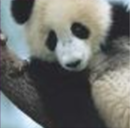
\includegraphics{adv_panda}

          \textbf{\blue{Prediction}}
          \\
          \textbf{Panda}
          \\
          55.7\% Confidence~\cite{Goodfellow:2014}
        \end{center}
      }
    \end{column}
    \onslide<+->{
      \begin{column}{0.05\textwidth}
          \begin{center}
            +\vspace{1.6cm}
          \end{center}
      \end{column}
      \begin{column}{0.20\textwidth}
          \begin{center}
            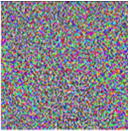
\includegraphics{adv_noise}

            \textbf{\blue{Prediction}}
            \\
            \textbf{Nematode}
            \\
            8.2\% Confidence
          \end{center}
      \end{column}
    }
    \onslide<+->{
      \begin{column}{0.05\textwidth}
          \begin{center}
            =\vspace{1.6cm}
          \end{center}
      \end{column}
      \begin{column}{0.20\textwidth}
          \begin{center}
            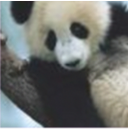
\includegraphics{adv_combined}
            \textbf{\blue{Prediction}}
            \\
            \textbf{Gibbon}
            \\
            99.3\% Confidence
          \end{center}
      \end{column}
    }
    \onslide<+->{
      \begin{column}{0.20\textwidth}
          \begin{center}
            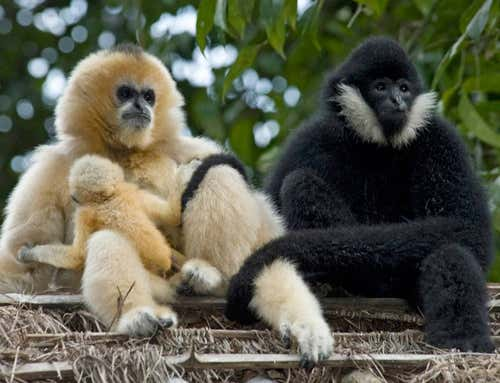
\includegraphics[scale=0.15]{gibbon}
            \textbf{\red{Actual}\\Gibbon}
          \end{center}
      \end{column}
    }
  \end{columns}

\end{frame}

\begin{frame}{$\ell_{p}$ Balls --- Norms First}
  For ${x \in \mathbb{d}}$, the $L_{p}$ norm is:

  \begin{equation}\label{eq:LpNorm}
    \norm{x}_{p} = \left( \sum_{i=1} x_{i}^{p}  \right)^{\frac{1}{p}}
  \end{equation}

  $L_{\infty}$ norm is a special a case:

  \begin{equation}\label{eq:LinftyNorm}
    \norm{x}_{\infty} = \sup_{i} \abs{x_i}
  \end{equation}

  \begin{center}
    \textbf{Note}: $\sup$ equals the $\max$ for a finite set
  \end{center}
\end{frame}

\begin{frame}{$\ell_{p}$ Balls --- Let's Visualize\ldots}
  \begin{definition}
    Given scalar ${\varepsilon > 0}$, the $\ell_{p}$ ball of a point ${x \in \mathbb{R}^{d}}$ is:

    \begin{equation}\label{eq:LpBall}
      \ell_{p}(x) = \setbuild{x + \delta}{\norm{\delta}_{p} \leq \varepsilon}\text{.}
    \end{equation}
  \end{definition}

  \onslide<+->{
    \begin{center}
      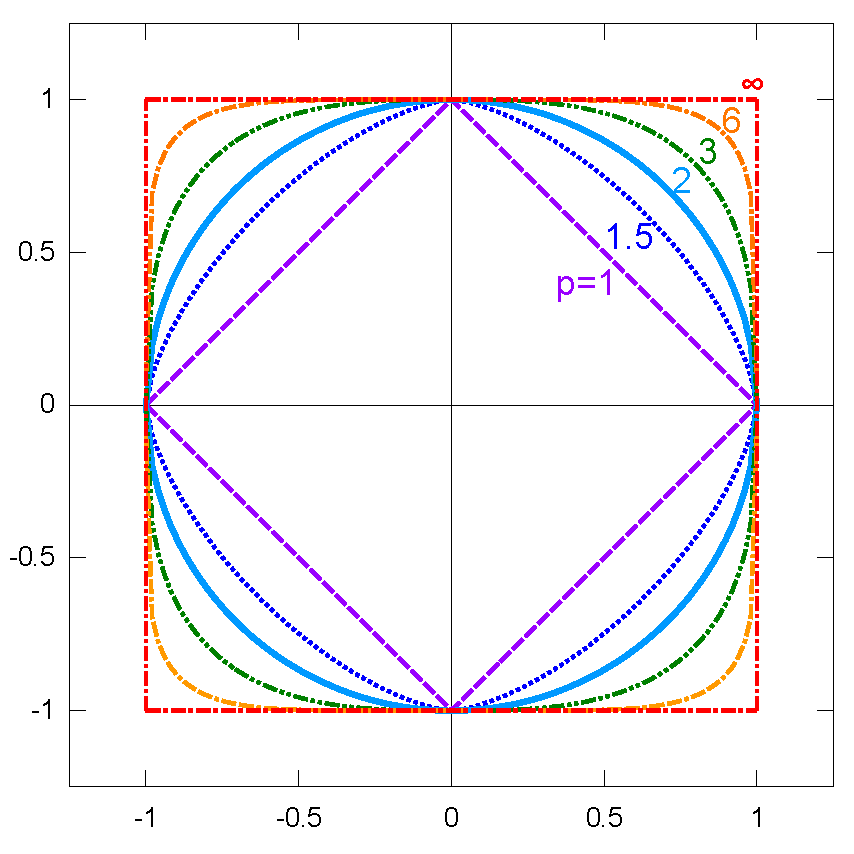
\includegraphics[scale=0.29]{img/lpballs.pdf} \cite{wiki:Lp_space}
    \end{center}
  }
\end{frame}


\begin{frame}{Attack Paradigms}
  \madry\ study adversarial robustness under two different attack paradigms:
  \vfill
  \begin{enumerate}[<+->]
    \item \textbf{Black-Box}: Adversary has no direct access to target network
      \begin{itemize}[<+->]
        \setlength\itemsep{6pt}
        \item \red{Weaker} attack paradigm
        \item Adversary may have \textit{rough} information, e.g.,~model architecture \& training dataset
          \begin{itemize}
            \item \textit{Example}: Transfer attack
          \end{itemize}
        \item Generally \textit{one-shot} attacks
      \end{itemize}
    \vfill
    \item \textbf{White-Box}: Attacker has access to target network's parameter
      \begin{itemize}
        \setlength\itemsep{6pt}
        \item \green{Stronger} attack paradigm
        \item \textit{Examples}: PGD and FGSM (both discussed in this talk)
        \item Enables \textit{iterative} attacks, e.g.,~refined probing
      \end{itemize}
  \end{enumerate}
\end{frame}


\begin{frame}{Nomenclature}
  \onslide<+->{Quite standard and used throughout this talk.}  \onslide<+->{\textit{If you have a question,} \textbf{ask now!}}

  \begin{itemize}[<+->]
    \setlength{\itemsep}{6pt}
    \item ${\X \in \domainX}$: feature values
    \item ${\y \in \domainY}$: Ground truth (true) label
    \item $\func{\distr}{\domainX \times \domainY}{\mathbb{R}_{{\geq}0}}$: Underlying sample data probability distribution s.t.\ ${(\X,\y) \sim \distr}$

    \vspace{6pt}
    \item ${\params \in \domainP}$: Model (neural network) parameters

    \vspace{6pt}
    \item ${\sPerturb \subseteq \domainX}$: Set of allowed (adversarial) perturbations can be applied to any~$\X$
    \item ${\perturb \in \sPerturb}$: (Adversarial) perturbation s.t.
      \begin{equation}\label{eq:AdversarialX}
        \X^{\text{adv}} = x + \delta
      \end{equation}

    \vspace{6pt}
    \item $\mathbb{E}_{x \in \mathcal{X}}\sbrack{f(x)}$: Expected value (weighted mean) of $f(x)$ for all ${x \in \mathcal{X}}$
  \end{itemize}
\end{frame}


\section{Optimization \& Adv.\ Robustness}
\transitionFrame{Relating Optimization \& Adversarial Guarantees}


\begin{frame}{What is an adversarial \blue{guarantee}?}
  \begin{itemize}[<+->]
    \setlength{\itemsep}{20pt}
    \item Last week we reviewed multiple possible defensive techniques, e.g.,~robustness, disinformation,~etc.
    \item \textbf{Guarantee}: Certifies that a ``well-defined'' class of adversarial attacks are prevented
      \begin{itemize}
        \item \textit{Example}: Class of \textbf{\blue{first-order adversaries}} (under certain conditions)
      \end{itemize}

    \item \textbf{Question}: What guarantees did the authors' of last week's paper provide?
    \vspace{-14pt}
    \item \textbf{Answer}: None. \onslide<+->{\textit{And that's the point}}
      \begin{itemize}[<+->]
        \item \textbf{\green{Goal}}: Make \textbf{\blue{provable statements about robustness}}.
        \item If we can do it, that's a yuge deal
      \end{itemize}
  \end{itemize}
\end{frame}


\begin{frame}{Nomenclature}
  \onslide<+->{Quite standard and used throughout this talk.}  \onslide<+->{\textit{If you have a question,} \textbf{ask now!}}

  \begin{itemize}[<+->]
    \setlength{\itemsep}{6pt}
    \item ${\X \in \domainX}$: feature values
    \item ${\y \in \domainY}$: Ground truth (true) label
    \item $\func{\distr}{\domainX \times \domainY}{\mathbb{R}_{{\geq}0}}$: Underlying sample data probability distribution s.t.\ ${(\X,\y) \sim \distr}$

    \vspace{6pt}
    \item ${\params \in \domainP}$: Model (neural network) parameters

    \vspace{6pt}
    \item ${\sPerturb \subseteq \domainX}$: Set of allowed (adversarial) perturbations can be applied to any~$\X$
    \item ${\perturb \in \sPerturb}$: (Adversarial) perturbation s.t.
      \begin{equation}\label{eq:AdversarialX}
        \X^{\text{adv}} = x + \delta
      \end{equation}

    \vspace{6pt}
    \item $\mathbb{E}_{x \in \mathcal{X}}\sbrack{f(x)}$: Expected value (weighted mean) of $f(x)$ for all ${x \in \mathcal{X}}$
  \end{itemize}
\end{frame}


\begin{frame}{``Standard'' Classification Model}
  \begin{itemize}[<+->]
    \setlength{\itemsep}{20pt}
    \item Neural network training is based on \textit{\blue{empirical risk minimization}} (ERM)
    \item \textbf{\green{Fundamental Idea}}:
      \begin{equation}\label{eq:ERM}
        \min_{\params} \mathbb{E}_{(\X,\y) \sim \distr} \sbrack{\loss \left( \X, \y ; \params \right)}
      \end{equation}

    \item \textit{\blue{Attack Model}}: For any ${x \in \domainX}$, adversary can make a set of allowed perturbations~$\sPerturb$
      \begin{itemize}
        \item \textit{Theoretical Paradigm}: $\sPerturb = \linf\text{-ball}$
      \end{itemize}

    \item \textbf{\red{Big Problem}}: ERM-trained models are not robust to adversarially perturbed examples~\cite{Biggio:2013,Szegedy:2013}
  \end{itemize}
\end{frame}


\subsection{Minimax}
\begin{frame}{Minimax Framework}
  \begin{definition}
    \blue{\textit{Minimax optimization}} reformulates ERM as:
    \onslide<2->{
      \begin{equation}\label{eq:Minimax}
        \textcolor<5->{ForestGreen}{\min_{\params} \rho(\params)}\text{, where } \rho(\params) = \mathbb{E}_{(\X,\y) \sim \distr} \sbrack{\textcolor<4->{red}{ \max_{\delta \in \sPerturb} \loss (\X + \perturb, \y ; \params)}} \text{.}
      \end{equation}
    }
  \end{definition}

  \vspace{8pt}
  \only<3-6>{Optimization Framework's Two Key Parts
    \begin{itemize}
      \setlength{\itemsep}{4pt}
    \item \onslide<4->{\textbf{\color{red}Inner Maximization}: Adversary finds (\textbf{worst case}) ${\xadv = \X + \perturb}$ with highest loss}
      \item \onslide<5->{\textbf{\color{ForestGreen}Outer Minimization}: Defender selects model parameters~$\params$ that minimize adversarial loss}
    \end{itemize}
  }
  \only<7->{
    \textbf{Question}: What can we say if ${\textcolor{ForestGreen}{\min_{\params} \rho(\params)} \rightarrow 0}$?

    \vspace{4pt}
    \onslide<8->{\textbf{Answer}: \green{Perfect robustness}. \textit{Security guarantee} no perturbation defined in attack model ($\sPerturb$) fools the network.}
    \begin{itemize}
      \item \onslide<9->{\textbf{Summary}: No adversarial examples!\textsuperscript{*}}
    \end{itemize}

    \vspace{10pt}
    \onslide<10->{\textbf{Why?}} \onslide<11->{Inner maximization considers \textbf{worst case} adversary guaranteeing all cases}
   }
\end{frame}


\begin{frame}{So\ldots Are We Done Here?}
  \onslide<+->{}
  \onslide<+->{\textbf{No.}} \onslide<+->{Inner \& outer components of minimax formulation are non-convex and non-concave respectively.}
  \vfill
  \onslide<+->{\textbf{\green{Key Contribution \#1}}: Demonstrating adversarial minimax optimization \textit{is} tractable.}
  \begin{itemize}[<+->]
    \item We will talk about tractability next.
  \end{itemize}
\end{frame}


\begin{frame}{Two Primary Questions}
  \onslide<+->{Previous work focused on two primary questions.  These form the basis of this work.}
  \vfill
    \begin{itemize}[<+->]
      \setlength\itemsep{15pt}
      \item How can we produce \textit{strong} adversarial examples that fool the model with high confidence while requiring only a small perturbation?

      \item How can we train a model so there are no \only<+->{(\textit{easily found}) }adversarial examples?
    \end{itemize}
  \vfill
  \onslide<+->{We will tackle these two questions separately with the first one being much more interesting}
\end{frame}

\section{Producing Strong Adversarial Examples}
\transitionFrame{Producing Strong Adversarial Examples}

\begin{frame}{Adversarial Examples should be Intractable}

  \onslide<+->{\textbf{\green{Inner Maximization}}: Adversarial example generation problem:
      \begin{equation}\label{eq:InnerMaximization}
        \max_{\delta \in \sPerturb} \loss (\X + \perturb, \y ; \params)
      \end{equation}

    \vspace{-3pt}
    is a highly non-concave function.  Potentially large number of local maxima making this problem \textit{seem} intractable.
  }

  \vfill
  \begin{itemize}[<+->]
    \setlength{\itemsep}{8pt}
    \item \textbf{\red{Previous Work}}: Fast Gradient Sign Method (FGSM)
  \end{itemize}
\end{frame}


\begin{frame}{Previous Work: Fast Gradient Sign Method}
  \onslide<+->{%
    \begin{definition}
      \textbf{\blue{Fast Gradient Sign Method}} (FGSM) linearizes the inner maximization s.t.:

      \begin{equation}\label{eq:FGSM}
        \xadv = \X + \varepsilon \sgn\left(\nabla_{\X} \loss(\X, \y ; \params) \right)
      \end{equation}
    \end{definition}
  }

  \begin{itemize}[<+->]
    \setlength\itemsep{8pt}
    \item \textbf{Summary}: Simple ``single-step-size'' approach
    \item Enhanced versions of FGSM (e.g., multi-step, randomized) that are beyond the scope of this talk
  \end{itemize}

  \vspace{3pt}
  \onslide<+->{\textbf{\red{Major Issue}}: FGSM provides no security guarantee}
  \begin{itemize}[<+->]
    \setlength\itemsep{8pt}
    \item \textbf{Why?} \onslide<+->{Not selecting the \textit{worst-case} perturbation}
    \item Easy to find ``nearby'' perturbations with significantly higher loss
  \end{itemize}
  \vfill
  \onslide<+->{\textbf{\madry's Solution}: \blue{\textbf{Projected Gradient Descent}} (PGD)}
\end{frame}


\begin{frame}{Projected Gradient Descent (PGD)}
  \onslide<+->{\textbf{Question}: What is PGD?}

  \vspace{4pt}
  \onslide<+->{\textbf{Answer}: Form of \green{\textit{constrained optimization}} where the constraint is a \blue{\textbf{projection}}}

  \vfill
  \onslide<+->{
    \begin{definition}
      A \textbf{\blue{projection}} of a point~$z$ onto a set~$\mathcal{X}$ is defined as:

      \[ \Pi_{\sPerturb}(z) = \argmin_{s \in \sPerturb} \norm{s-z}_{p}\text{.}  \]
    \end{definition}
  }

  \vfill
  \begin{itemize}[<+->]
    \item $\Pi_{\sPerturb}$ is the projection operator
  \end{itemize}
\end{frame}


\begin{frame}{Projected Gradient Descent --- The Algorithm}
  \begin{columns}
    \begin{column}{0.5\textwidth}
      \textbf{Procedure}:
      \begin{enumerate}[<+->]
        \setlength{\itemsep}{12pt}
        \item For any ${\X \in \mathcal{X}}$, define ${\X^{(0)} = \X + \perturb}$ where ${\perturb \sim \mathcal{U}\left( \sPerturb \right)}$
        \item At each time $t$, define:
          \begin{equation}\label{eq:PGD:GradUpdate}
            z^{(t+1)} = \X^{(t)} \textcolor<6->{red}{-} \alpha \nabla_{\X} \loss(\X^{(t)}, \y) \text{.}
          \end{equation}
        \item Enforce the constraint where:
          \begin{equation}\label{eq:PGD:NextX}
            \X^{(t+1)} = \Pi_{\sPerturb}(z^{(t+1)}) \text{.}
          \end{equation}

        \item Repeat steps~\#2 and~\#3 until convergence
      \end{enumerate}
    \end{column}
    \begin{column}{0.45\textwidth}
      \begin{center}
        \onslide<+->{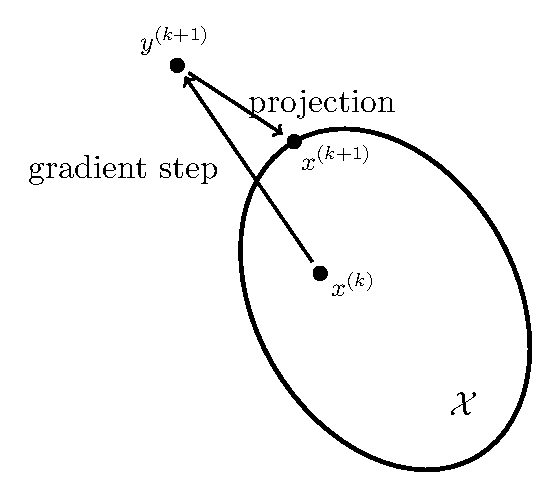
\includegraphics[scale=0.65]{pgd}~\cite{Srebro}}
      \end{center}
    \end{column}
  \end{columns}
\end{frame}

\subsection{\texorpdfstring{$\ell_{p}$}{Lp}-Balls}

\begin{frame}{What is our constraint set~$\sPerturb$?}
  \begin{itemize}[<+->]
    \setlength{\itemsep}{20pt}
    \item By definition, PGD requires a constraint set,~$\sPerturb$

    \item Recall that in adversarial training,~$\sPerturb$, is the set of allowed perturbations

    \item In this paper, $\sPerturb$ is an $\ell_{p}$-ball
      \begin{itemize}
        \item Let's define what those are\ldots
      \end{itemize}
  \end{itemize}
\end{frame}


\begin{frame}{$\ell_{p}$-Balls --- Norms First}
  \onslide<+->{For ${x \in \mathbb{R}^d}$, the $L_{p}$ norm is:}

  \onslide<+->{%
    \begin{equation}\label{eq:LpNorm}
      \norm{x}_{p} = \left( \sum_{i=1} x_{i}^{p}  \right)^{\frac{1}{p}}
    \end{equation}
  }

  \onslide<+->{$L_{\infty}$ norm is a special case:}

  \onslide<+->{%
    \begin{equation}\label{eq:LinftyNorm}
      \norm{x}_{\infty} = \sup_{i} \abs{x_i}
    \end{equation}
  }

  \onslide<+->{%
    \begin{center}
      \textbf{Note}: ``$\sup$'' equals the ``$\max$'' for a finite set
    \end{center}
  }
\end{frame}

\begin{frame}{$\ell_{p}$-Balls --- Formally}
  \begin{definition}
    Given scalar ${\varepsilon > 0}$, the $\ell_{p}$~ball of a point ${x \in \mathbb{R}^{d}}$ is the set:

    \begin{equation}\label{eq:LpBall}
      \ell_{p}(x) = \setbuild{x + \delta}{\norm{\delta}_{p} \leq \varepsilon}\text{.}
    \end{equation}
  \end{definition}

  \begin{columns}
    \begin{column}{0.5\textwidth}
      \onslide<2->{Let's visualize $\ell_{p}$ for different values of $p$}

      \vspace{15pt}
      \onslide<4->{\blue{\textbf{Question}}: What is the value of $\varepsilon$?}

      \vspace{4pt}
      \onslide<5->{\textbf{Answer}: $\varepsilon = 1$}

      \vspace{15pt}
      \onslide<6->{\green{\textbf{Key Takeaway}}: $\ell_{\infty}$~ball is a superset of all other $\ell_{p}$~balls for fixed $\varepsilon$}
    \end{column}
    \begin{column}{0.45\textwidth}
      \onslide<3->{
        \begin{center}
          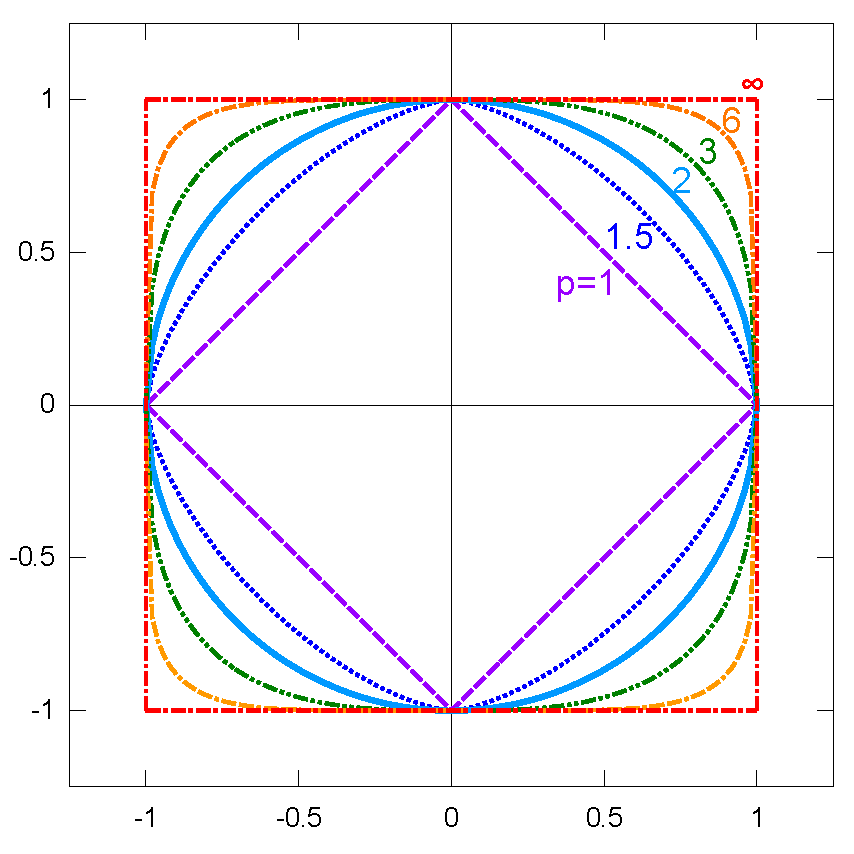
\includegraphics[scale=0.28]{img/lpballs.pdf}~\cite{wiki:Lp_space}
        \end{center}
      }
    \end{column}
  \end{columns}
\end{frame}


\subsection{\texorpdfstring{$\ell_{\infty}$}{L-infinity}~Ball \& PGD}

\begin{frame}{Connecting $\ell_{\infty}$ \& PGD}
  \begin{itemize}[<+->]
    \setlength{\itemsep}{20pt}
    \item Since ${\forall_{p \in \mathbb{R}} \hspace{3pt} \ell_p \subset \ell_{\infty}}$, providing an adversarial guarantee over $\ell_{\infty}$ guarantees that for any other $p$, the maximum loss will be the same or smaller.

    \item Uses complete first-order information, i.e.,~not only the gradient's information

    \item \textbf{Summary}: Training a network robust to PGD~adversaries makes it robust against a wide range of other attacks as well
  \end{itemize}
\end{frame}

\begin{frame}{PGD \& Adversarial Tractability}
  \onslide<+->{\textbf{\blue{Question}}: Is PGD + $\ell_{\infty}$\-/balls guaranteed to eliminate \textit{all} adversarial examples within (Minkowski) distance~$\varepsilon$ of $\X$?}

  \vspace{3pt}
  \onslide<3->{\textbf{Answer}: No.} \only<4-5>{Why?}
  \begin{itemize}
    \item \onslide<5->{PGD is only a \textbf{first-order adversary}.}
  \end{itemize}

  \vfill
  \onslide<6->{
    \begin{definition}
      \blue{\textbf{First-order adversary}} is the strongest attack utilizing only \textit{first-order} (e.g.,~gradient) information about network
    \end{definition}
  }

  \vfill
  \onslide<7->{An attacker using higher order information (e.g.,~Hessian) may tractably find adversarial examples.} \onslide<8->{They may even find them \textit{easily}.}
  \begin{itemize}
    \item \onslide<9->{Similar to \textit{polynomially-bounded} adversary that is cornerstone of cryptography}
  \end{itemize}
\end{frame}

\subsection{Zero-Order Adversaries}
\begin{frame}{Zero-Order Adversaries}
  \begin{itemize}[<+->]
    \setlength{\itemsep}{20pt}
    \item A \blue{\textbf{zero-order adversary}} has no direct access to the classifier and is only able to evaluate the classifier based on chosen examples
      \begin{itemize}
        \setlength{\itemsep}{8pt}
        \item ``Zero-order'' means no access to ``first-order'' information
        \item \textit{Translation}: \red{No gradient feedback}
      \end{itemize}

    \item \textit{Example}: Black-box attack

    \item Much more challenging that first-order attack
  \end{itemize}
\end{frame}


\section{Adversarial Example Landscape}
\transitionFrame{Adversarial Example Landscape}

\begin{frame}{Investigating the ``Inner Maximization''}
  \onslide<+->{%
    \begin{equation}
      \min_{\params} \rho(\params) \text{, where } \rho(\params) = \mathbb{E}_{(\X,\y) \sim \distr} \sbrack{\red{\max_{\delta \in \sPerturb} \loss (\X + \perturb, \y ; \params)}}
    \end{equation}
  }

  \begin{itemize}[<+->]
    \setlength{\itemsep}{20pt}
    \item Preceding theoretical analysis of \textbf{\red{inner maximization}} described PGD's usefulness to provide guarantees regarding first-order adversaries
    \item \textbf{Goal of this Section}: Demonstrate \textit{empirically} that the theoretical analysis holds even in environments that are theoretically \textit{intractable}
      \begin{itemize}[<+->]
        \setlength{\itemsep}{8pt}
        \item \textbf{Recall}: Inner maximization is highly \textit{non-concave} and not continuously-differentiable
        \item \textbf{Question}: Why are we interested in concavity and not convexity?
      \end{itemize}
  \end{itemize}
\end{frame}


\begin{frame}{Experimental Setup}
  \onslide<+->{Setup applies for all experiments in this section}
  \begin{itemize}[<+->]
    \setlength{\itemsep}{10pt}
    \item \textbf{Datasets}: MNIST \& CIFAR10

    \item \textbf{Procedure}: Select example,~$\X$, u.a.r.\ from the dataset, then for each random restart:
      \begin{enumerate}[<+->]
        \setlength\itemsep{6pt}
        \item Select initial perturbation,~${\perturb \in \sPerturb}$, u.a.r.
        \item Perform PGD on perturbed example, ${\X + \perturb}$
      \end{enumerate}

    \item \textbf{\# Random Restarts}: Varies by experiment

    \item \textbf{Loss Function}: Cross-entropy
      \onslide<+->{
        \begin{equation}\label{eq:CrossEntropy}
          \loss(y,\hat{y}) = \sum_{c \in \mathcal{C}} -y_c \log \left( \hat{y}_{c} \right)
        \end{equation}
      }
  \end{itemize}
\end{frame}


\begin{frame}{Experiment~\#1: $\Delta\loss$ vs.\ \#Iterations}
  \onslide<+->{\textbf{Goal}: Study change in adversarial loss for each iteration of PGD}
  \begin{itemize}[<+->]
    \item \textbf{\# Random Restarts}: 20
  \end{itemize}

  \begin{columns}
    \begin{column}{0.23\textwidth}
      \begin{center}
        \onslide<+->{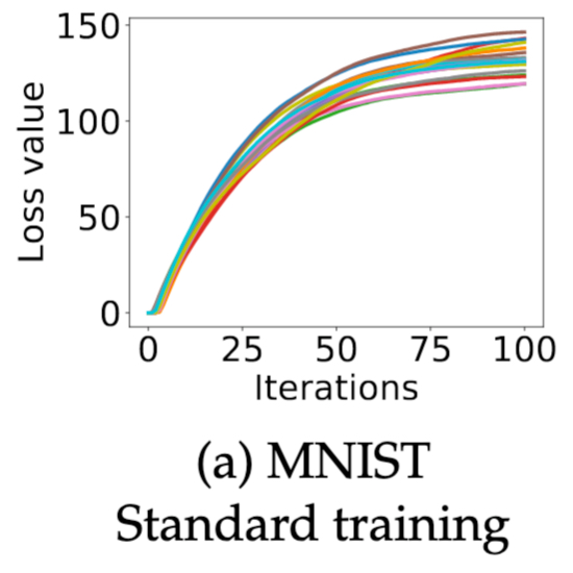
\includegraphics[scale=0.32]{loss_v_iter/mnist_standard.pdf}}
      \end{center}
    \end{column}
    \begin{column}{0.2\textwidth}
      \begin{center}
        \onslide<+->{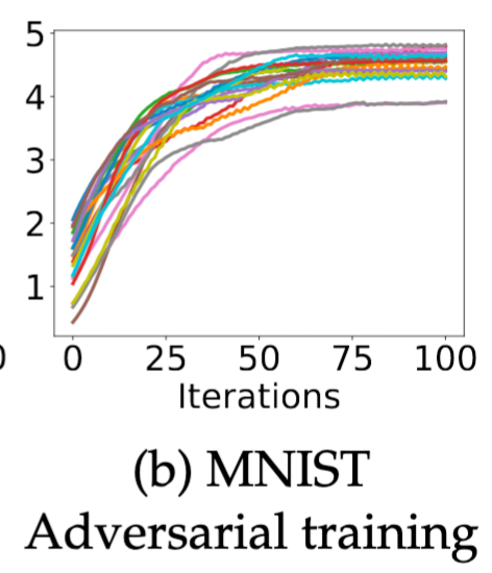
\includegraphics[scale=0.32]{loss_v_iter/mnist_adv.pdf}}
      \end{center}
    \end{column}
    \begin{column}{0.21\textwidth}
      \begin{center}
        \onslide<+->{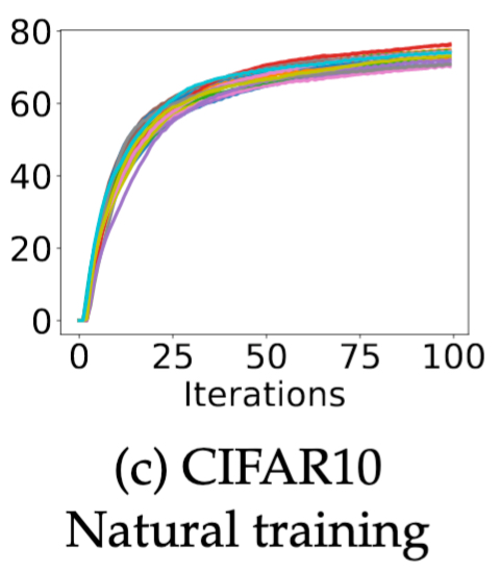
\includegraphics[scale=0.32]{loss_v_iter/cifar_standard.pdf}}
      \end{center}
    \end{column}
    \begin{column}{0.22\textwidth}
      % \vspace{-9pt}
      \begin{center}
        \onslide<+->{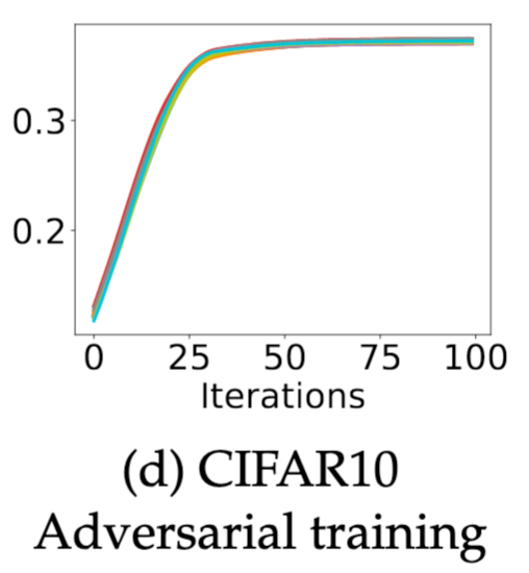
\includegraphics[scale=0.32]{loss_v_iter/cifar_adv.pdf}}
      \end{center}
    \end{column}
  \end{columns}
  \vfill
  \onslide<+->{\green{\textbf{Takeaways}}}
  \begin{itemize}[<+->]
    \item Adversarial training significantly reduces loss on adversarial examples.
    \item Loss values are \textbf{\blue{well-concentrated}}
      \begin{itemize}
        \item Echoes \textit{folklore belief} that neural network training possible since many local minima with similar loss values
      \end{itemize}
  \end{itemize}
\end{frame}


\begin{frame}{Experiment~\#2: Absence of Outliers}
  \onslide<+->{\textbf{Goal}: Verify security guarantee across many examples \& random restarts}
  \begin{itemize}[<+->]
    \item \textbf{\# Examples} ($x$): 5
    \item \textbf{\# Random Restarts}: 100K
  \end{itemize}

  \vspace{-15pt}
  \begin{columns}
    \begin{column}{0.7\textwidth}
      \begin{center}
        \onslide<4->{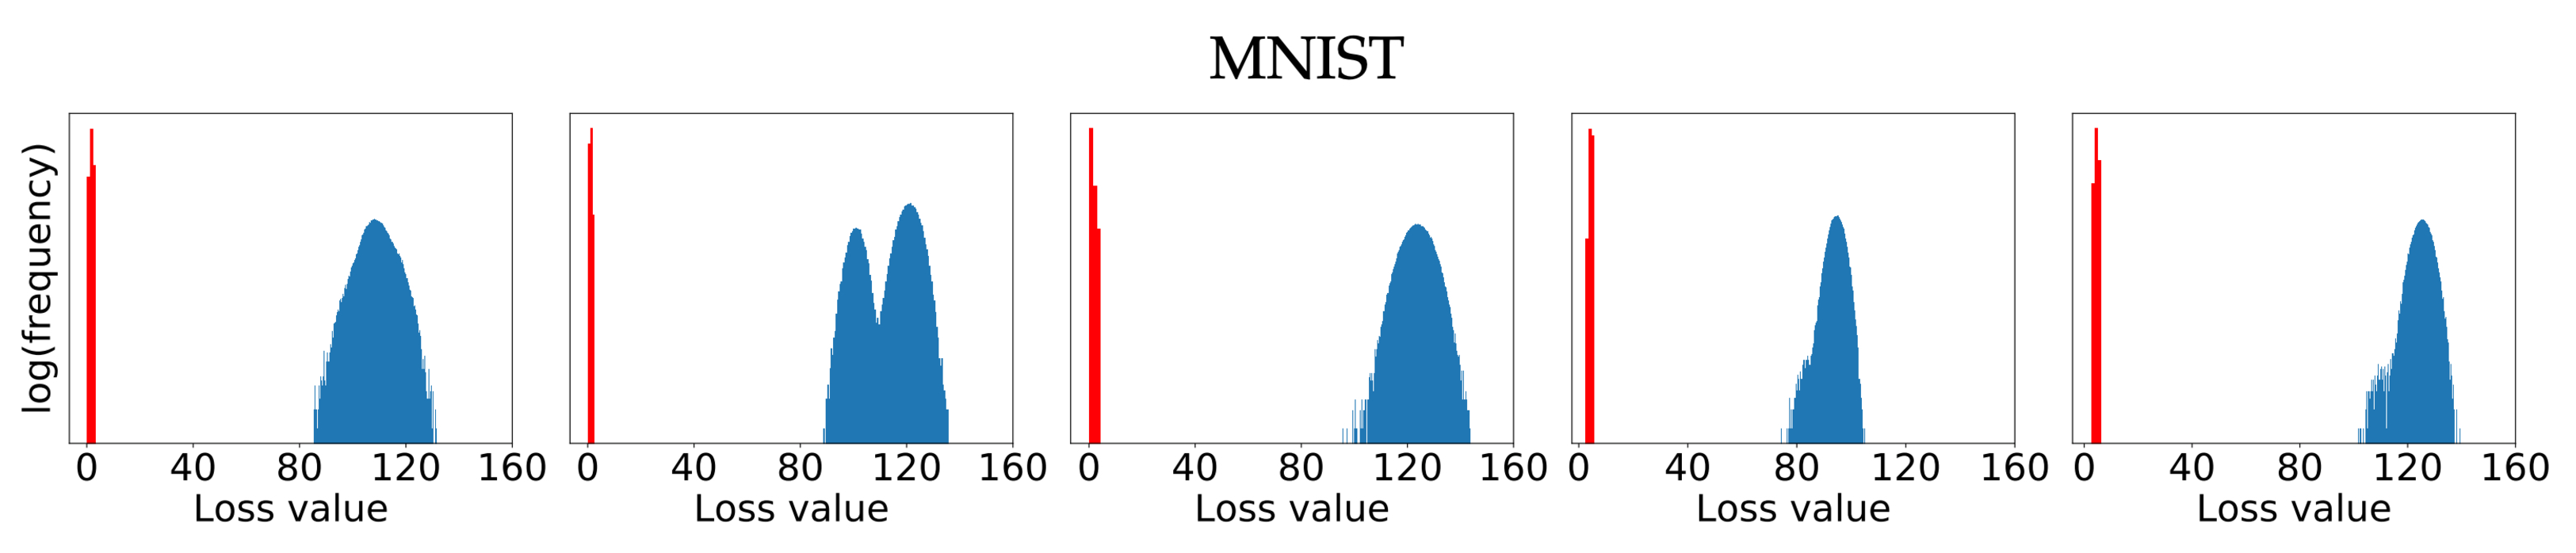
\includegraphics[scale=0.19]{loss_hist/mnist}}

        \onslide<6->{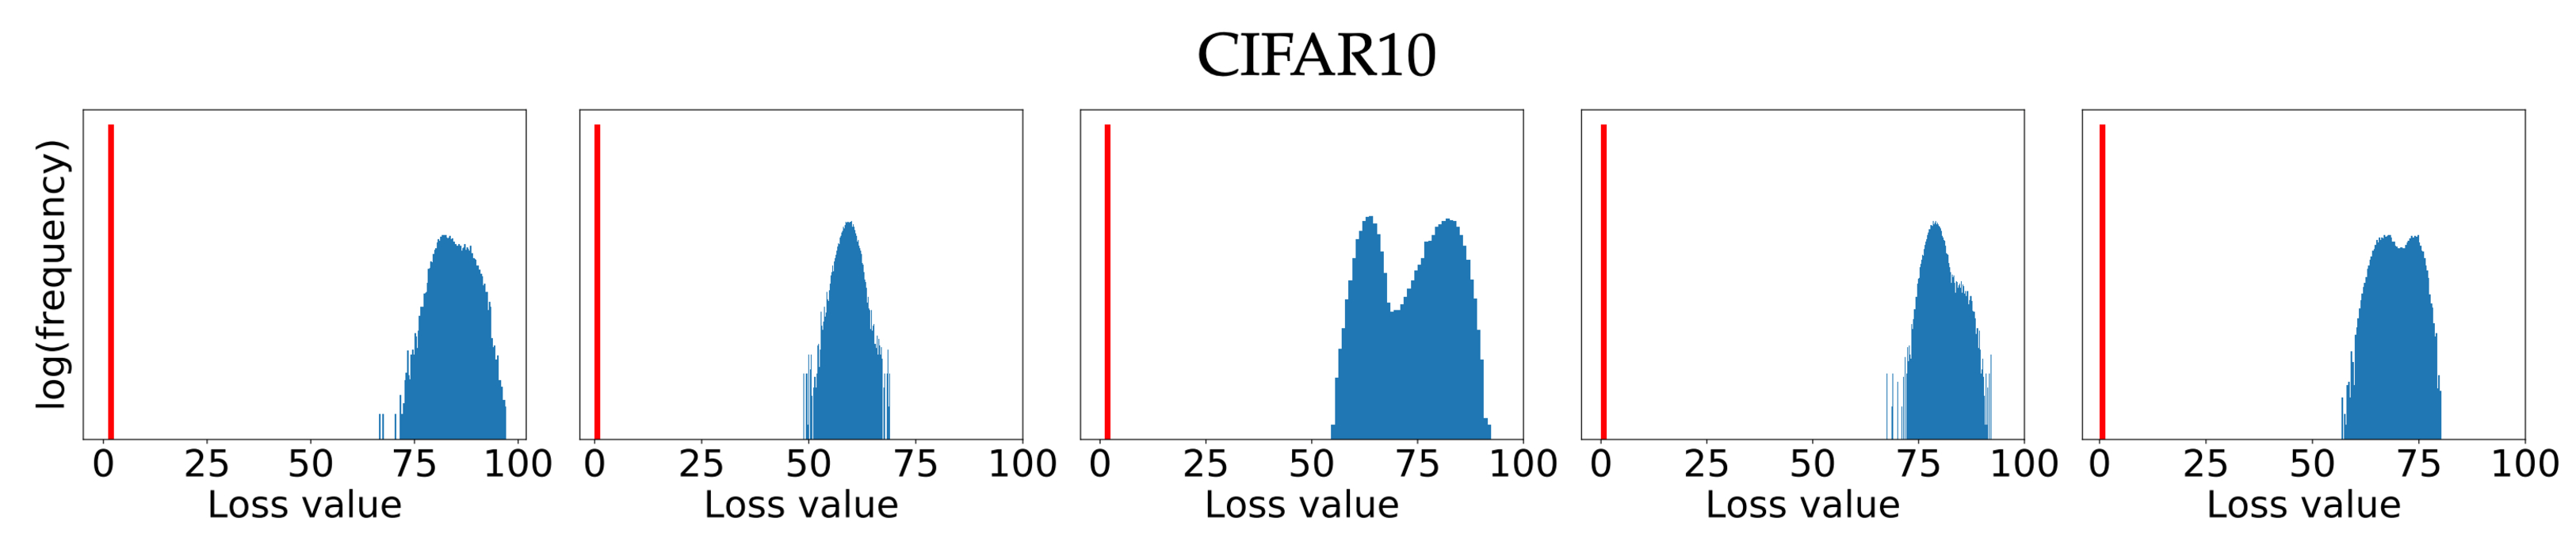
\includegraphics[scale=0.19]{loss_hist/cifar}}
      \end{center}
    \end{column}
    \begin{column}{0.25\textwidth}
      \vspace{20pt}
      \onslide<5->{
        \begin{itemize}
          \setlength{\itemsep}{20pt}
          \item \textbf{\blue{Blue}}: Standard training
          \item \textbf{\red{Red}}: Adversarial training
        \end{itemize}
      }
    \end{column}
  \end{columns}

  \vfill
  \onslide<7->{\green{\textbf{Takeaway}}: No outliers (i.e., high loss adversarial examples) \& concentrated losses}
\end{frame}


\begin{frame}{Experiment~\#3: ``Mode Collapse''}
  \onslide<+->{\textbf{\blue{Mode Collapse}}: Common problem in GANs where the generated outputs have limited diversity.}
  \vfill
  \onslide<+->{\textbf{Goal}: Demonstrate that the generated adversarial examples are noticeably distinct:}
  \begin{itemize}[<+->]
    \item \textbf{\# Random Restarts}: 10,000
    \item \textbf{Metric}: Inter-adversarial example (Euclidean) distance
  \end{itemize}
  \vfill
  \onslide<+->{\textbf{\green{Result}}: Inter-maxima distance is distributed close to the expected distance between \textit{two random points} in the $\ell_{\infty}$\-/ball and cosine similarity between points is close to 90\textsuperscript{$\circ$}.}
  \begin{itemize}[<+->]
    % \item Empirically demonstrates no adversarial example ``mode collapse''
    \item Recall the ``curse of dimensionality'' so take with a grain of salt
  \end{itemize}
  \vfill
  \onslide<+->{\textbf{\green{Takeaway}}: No evidence of mode collapse}
\end{frame}


\section{Adversarial Training}

\transitionFrame{Adversarially Robust Training}

\begin{frame}{Solving the Outer Minimization}
  \onslide<+->{%
    \begin{equation}\label{eq:MinimaxTrainRepeat}
      \green{\min_{\params} \rho(\params)} \text{, where } \rho(\params) = \mathbb{E}_{(\X,\y) \sim \distr} \sbrack{\red{\max_{\delta \in \sPerturb} \loss (\X + \perturb, \y ; \params)}}
    \end{equation}
  }

  \begin{itemize}[<+->]
    \item So far, we have only talked about solving the \red{inner maximization} to create adversarial examples

    \vspace{13pt}
    \item \textbf{Question}: What do we need to solve to train adversarially robust networks?
    \vspace{5pt}
    \item \textbf{Answer}: Solve the \green{outer minimization}

    \vspace{13pt}
    \item \textbf{Question}: What algorithm can use to solve the outer maximization?
    \vspace{5pt}
    \item \textbf{Answer}: Stochastic gradient descent (SGD) on the adversarial examples
      \begin{itemize}[<+->]
        \setlength{\itemsep}{6pt}
        \item \textit{Intuition}: SGD on adv.\ examples' loss reduces the \red{inner maximization}
        \item \textit{Takeaway}: Given an algorithm that transforms training examples into adv.\ examples (e.g.,~PGD), the rest of the \textbf{\blue{training process proceeds normally}}
      \end{itemize}
  \end{itemize}
\end{frame}


\begin{frame}{Why Should I Believe the Preceding Claims are True?}
  \onslide<+->{}
  \onslide<+->{\textbf{Answer}: You shouldn't.  The preceding explanation is definitely \red{not a proof}.}

  \vspace{20pt}
  \onslide<+->{\madry\ rely on \textbf{\blue{Danskin's Theorem}} that states gradients at inner maximizers (think adversarial examples) correspond to descent directions for the complete problem}

  \vspace{20pt}
  \onslide<+->{\textbf{Problem}: Multiple assumptions made by Danskin's Theorem's \red{do not apply} here, e.g.,~continuously differentiable function, only approximate inner maximizers etc.}
  \begin{itemize}[<+->]
    \setlength{\itemsep}{6pt}
    \item Empirical results show that despite Danskin's not holding the algorithm is addressing the issues
    \item A more complete discussion of how Danksin's applies to this problem is in Appendix~A (see Arxiv version) and is beyond the scope of this talk
  \end{itemize}
\end{frame}


\section{Network Capacity \& Adversarial Robustness}
\transitionFrame{Network Capacity \& Adversarial Robustness}

\begin{frame}
	\onslide<+->{Solving the following equation is not enough to guarantee the robustness and accuracy of the classifier.
		\begin{equation*}
		{\min_{\params} \rho(\params)}\text{, where } \rho(\params) = \mathbb{E}_{(\X,\y) \sim \distr} \sbrack{{ \max_{\perturb \in \sPerturb} \loss (\X + \perturb, \y ; \params)}}
		\end{equation*}
	}

	\onslide<+->{The problem must have a small \colortext{green}{\textit{value}}, which means that the final loss achieved by the classifier against adversarial examples must be small.}

	\vspace{4pt}

	\onslide<+->{Therefore, a very small \colortext{blue}{$\rho(\params)$} corresponds to a perfect classifier that is robust to adversarial inputs.}

	\vspace{4pt}

	\onslide<+->{For a fixed set $\sPerturb$, the value of the problem is entirely dependent on the
		architecture of the classifier.}

	\vspace{4pt}

	\onslide<+->{Therefore, the architectural capacity of the model is very important for its over performance.}
\end{frame}

\begin{frame}{Visualizing the Effect of Capacity}
	\begin{columns}
		\begin{column}{0.32\textwidth}
			\onslide<+->{
				\begin{center}
					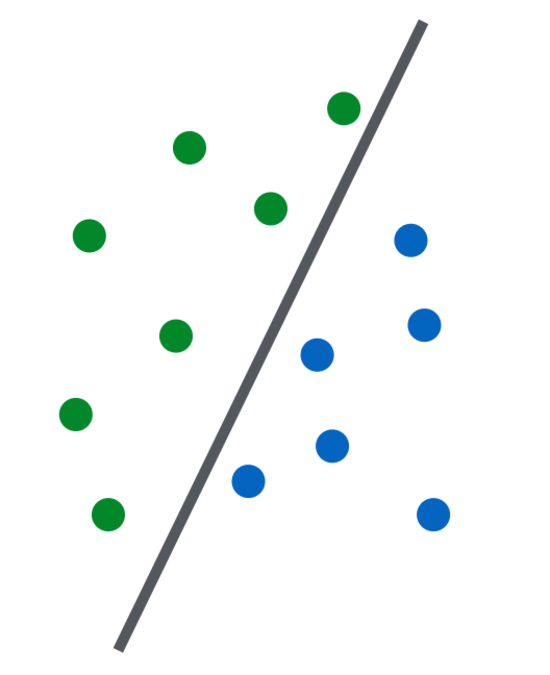
\includegraphics[scale=0.3]{capacity/benign_only.pdf}

					(Benign) binary classification using a \\\blue{linear decision boundary}
				\end{center}
			}
		\end{column}
		\begin{column}{0.32\textwidth}
			\onslide<+->{
				\begin{center}
					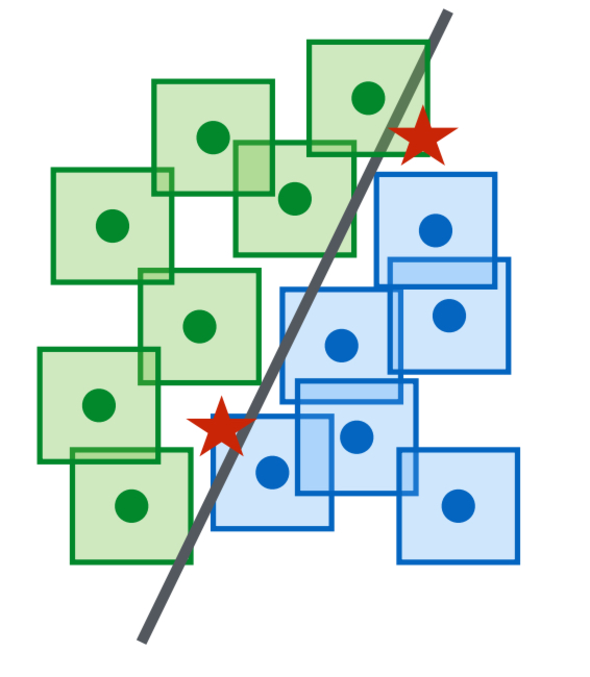
\includegraphics[scale=0.3]{capacity/misclassified_adv.pdf}

					Adversarial $\ell_{\infty}$ balls
					\\
					\red{$\star$} misclassified \\ adversarial examples
				\end{center}
			}
		\end{column}
		\begin{column}{0.32\textwidth}
			\onslide<+->{
				\begin{center}
					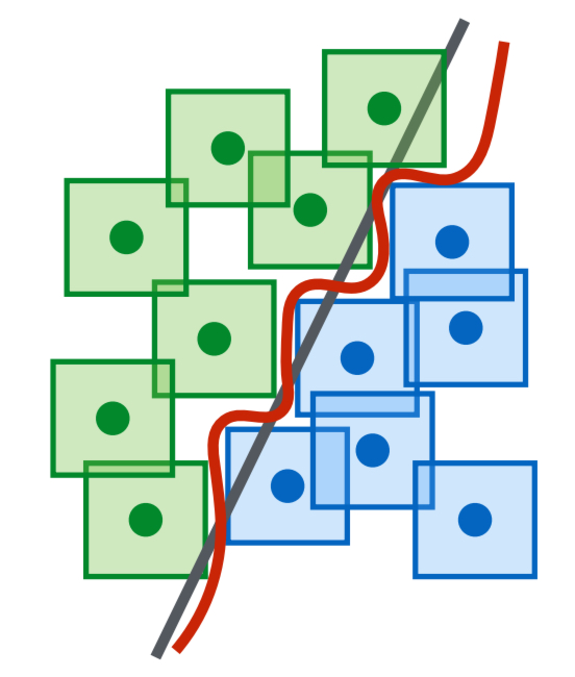
\includegraphics[scale=0.3]{capacity/complicated_decision.pdf}

					``Complicated'' decision boundary required
				\end{center}
			}
		\end{column}
	\end{columns}
\end{frame}

\begin{frame}{}
	\begin{columns}
		\begin{column}{0.48\textwidth}
			\onslide<+->{
				\begin{center}
					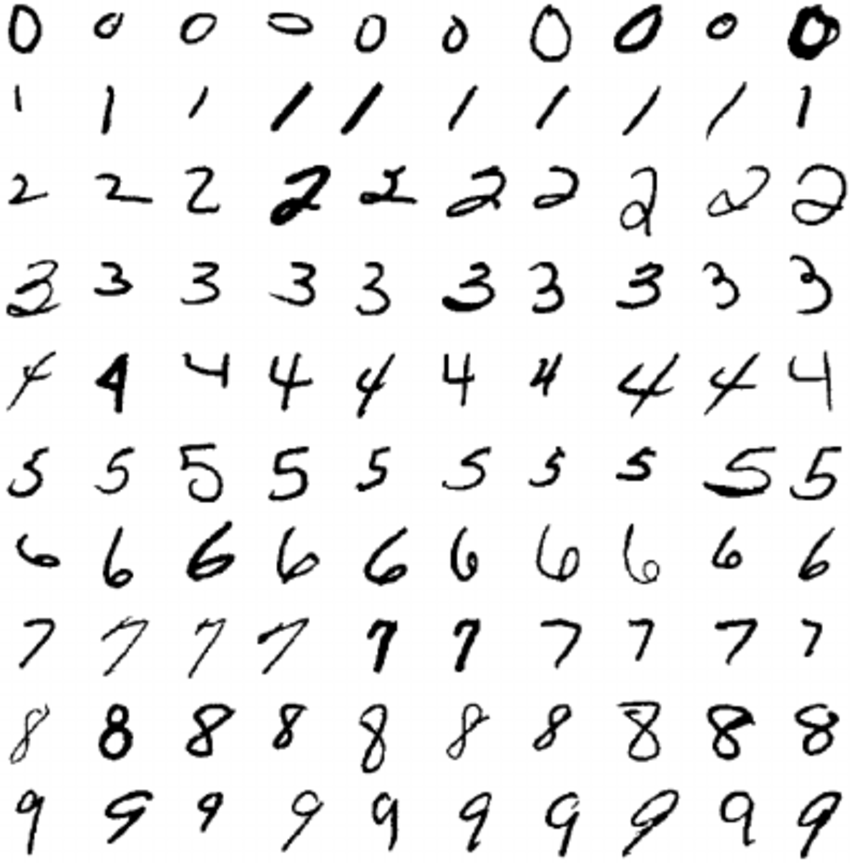
\includegraphics[scale=0.18]{nc_ar/mnist.png}

					MNIST
				\end{center}
			}
		\end{column}
		\begin{column}{0.48\textwidth}
			\onslide<+->{
				\begin{center}
					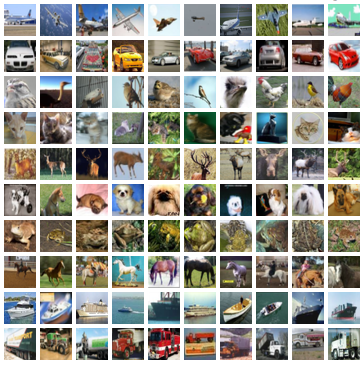
\includegraphics[scale=0.44]{nc_ar/cifar10.png}

					CIFAR10
				\end{center}
			}
		\end{column}
	\end{columns}
\end{frame}

\begin{frame}
	\onslide<+->{Verified by their experiments, capacity is crucial for:
		\begin{itemize}[<+->]
			\setlength\itemsep{8pt}
			\item Robustness
			\item The ability to successfully train a classifier against strong adversaries.
		\end{itemize}
	}
	\begin{columns}
		\begin{column}{0.99\textwidth}
			\onslide<+->{
				\begin{center}
					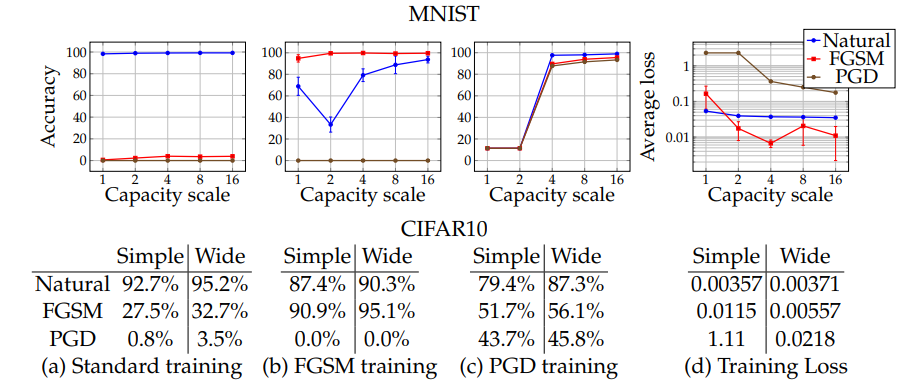
\includegraphics[scale=0.38]{nc_ar/fig4.png}
				\end{center}
			}
		\end{column}
	\end{columns}
\end{frame}

\begin{frame}
	\onslide<+->{What they found:
		\begin{itemize}[<+->]
			\setlength\itemsep{3pt}
			\item Capacity alone helps
				\begin{itemize}[<+->]
					\setlength\itemsep{1pt}
					\item Even with training on natural examples, increase in capacity increases the robustness against one-step perturbation
					\item  This effect is greater when considering adversarial examples with smaller $\varepsilon$
				\end{itemize}
			\item FGSM adversaries don’t increase robustness (for large  $\varepsilon$)
			\begin{itemize}[<+->]
				\setlength\itemsep{1pt}
				\item Training a network with FGSM adversaries and large  $\varepsilon$ results in
				\item Known as label leaking
				\item For smaller $\varepsilon$, FGSM adversaries are close to PGD, which makes it reasonable
			\end{itemize}
			\item Weak (small capacity) models may fail to learn non-trivial classifiers
			\begin{itemize}[<+->]
				\setlength\itemsep{1pt}
				\item Even though the model could converge to an accurate classifier through standard training, it is sacrificed for any kind of robustness against adversarial inputs
				\item But the model is still vulnerable to attacks
			\end{itemize}
			\item The value of the saddle point problem decreases as we increase the capacity
			\item More capacity and stronger adversaries decrease transferability
			\begin{itemize}[<+->]
				\setlength\itemsep{1pt}
				\item Otherwise, tranferability results in vulnerability to attacks even when there is no direct access to the target network
			\end{itemize}
		\end{itemize}
	}
\end{frame}

\subsection{Experiments}
\begin{frame}
	\onslide<+->{Two key elements in training their robust classifiers
		\begin{itemize}[<+->]
			\setlength\itemsep{8pt}
			\item A sufficiently high capacity network
			\item The strongest possible adversary
		\end{itemize}
	}
	\vspace{15pt}
	\onslide<+->{Using a "complete" first-order adversary by PGD for both MNIST and CIFAR10:
		\begin{itemize}[<+->]
			\setlength\itemsep{8pt}
			\item Multiple epochs for training the model. Therefore, no benefit from restarting PGD multiple times per batch
		\end{itemize}
	}
\end{frame}


\begin{frame}
	The steady decrease in the training loss of adversarial examples indicates the successfulness of the solution for the original optimization problem during training.

	\begin{columns}
		\begin{column}{0.99\textwidth}
			\onslide<+->{
				\begin{center}
					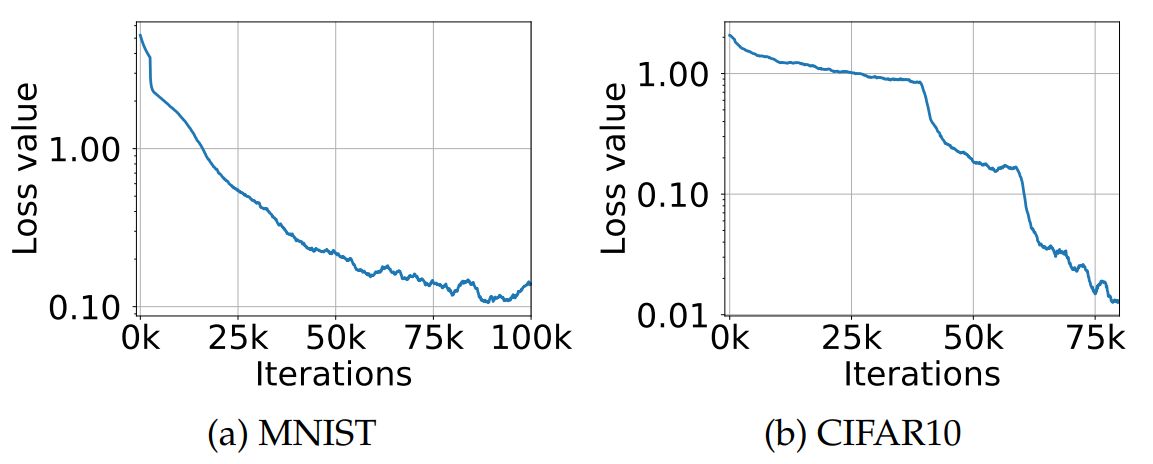
\includegraphics[scale=0.3]{nc_ar/fig5.png}
				\end{center}
			}
		\end{column}
	\end{columns}
\end{frame}

\begin{frame}
	\onslide<+->{Models are trained against a range of adversaries:
		\begin{itemize}[<+->]
			\setlength\itemsep{4pt}
			\item White-box attacks with PGD for a different number of iterations and restarts (A)
			\item White-box attacks with PGD using the Carlini-Wagner (CW) \cite{tramer2017space}, and CW+ when ${\kappa = 50}$ (i.e. attack with a high confidence)
			\begin{itemize}[<+->]
				\setlength\itemsep{4pt}
				\item ${f(x^{'}) = max(max\{Z(x^{'})_{i}: i \neq t\} - Z(x^{'})_{t}, -\kappa)}$
				\item z is the output of all layers except the softmax in a NN (so z is the logit)
			\end{itemize}
			\item Black-box attacks from an independently trained copy of the network (A$^{'}$).
			\item Black-box attacks from a version of the same network trained only on natural examples (A$_{nat}$)
			\item Black-box attacks from a different convolution architecture (B)
		\end{itemize}
	}
\end{frame}

\begin{frame}
	\begin{columns}
		\begin{column}{0.48\textwidth}
			\onslide<+->{
				\begin{center}
					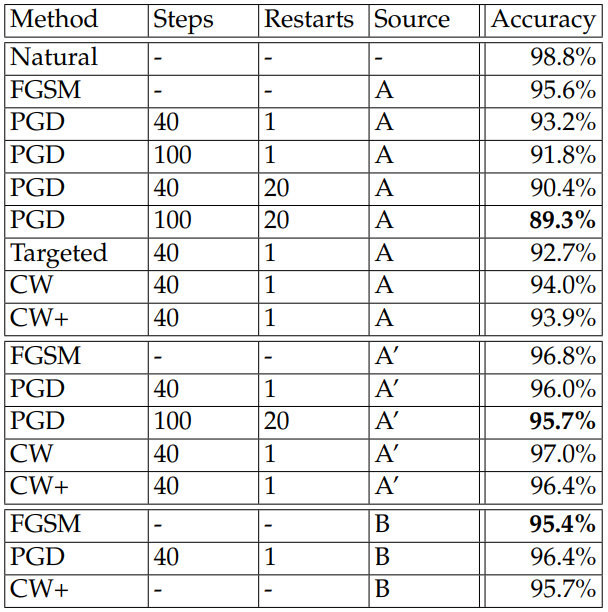
\includegraphics[scale=0.3]{nc_ar/table1.png}
					MNIST
				\end{center}
			}
		\end{column}
		\begin{column}{0.48\textwidth}
			\onslide<+->{
				\begin{center}
					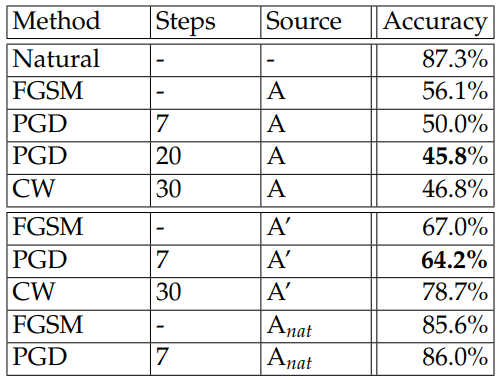
\includegraphics[scale=0.4]{nc_ar/table2.png}
					CIFAR10
				\end{center}
			}
		\end{column}
	\end{columns}
\end{frame}

\begin{frame}
	Resistance for different values of $\varepsilon$ and $\ell_{2}$-bounded attacks
	\begin{columns}
		\begin{column}{0.99\textwidth}
			\onslide<+->{
				\begin{center}
					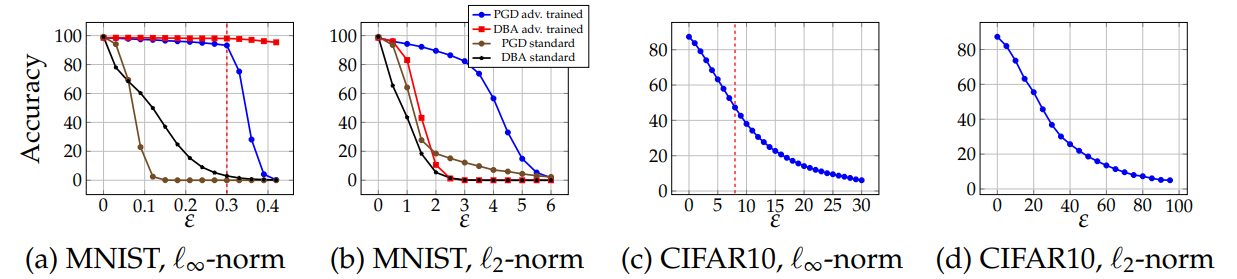
\includegraphics[scale=0.3]{nc_ar/fig6.png}
				\end{center}
			}
		\end{column}
	\end{columns}
\end{frame}

\begin{frame}
	\onslide<+->{Conclusion:
		\begin{itemize}[<+->]
			\setlength\itemsep{15pt}
			\item Although deep neural networks very vulnerable to adversarial attacks, they can be made resistant to adversarial attacks
			\item Based on the theory and experiments, reliable adversarial training methods can be designed because of the unexpectedly regular structure of the underlying optimization task:
			\begin{itemize}[<+->]
				\setlength\itemsep{15pt}
				\item Even though the relevant problem corresponds to the maximization of a highly
				non-concave function with many distinct local maxima, their values are highly concentrated.
			\end{itemize}
		\end{itemize}
	}
\end{frame}

\section{Related Works}
\begin{frame}
	\begin{itemize}[<+->]
		\setlength\itemsep{15pt}
		\item Robust optimization, not a new topic
		\item Adversarial ML, not a new topic
		\item Having the above in the context of DNN is their contribution
	\end{itemize}
	\vspace{8pt}
	\onslide<+->{
		Recent work on adversarial training on ImageNet also observed that the model capacity is important for adversarial training.
	}
	\vspace{8pt}

	\onslide<+->{
		( Their contribution) Training against multi-step methods (PGD) does lead to resistance against adversaries
	}
\end{frame}

\begin{frame}
	\onslide<+->{
		There are previous works on the min-max optimization problem. But, there are three differences:
		\begin{itemize}[<+->]
			\setlength\itemsep{15pt}
			\item (Previous works) the inner maximization problem can be difficult to solve, (they) it
			is possible to obtain sufficiently good solutions using randomly re-started projected gradient descent
			\item (Previous works) one-step adversaries, (they) multi-step methods
			\item (Previous works)  FGSM --FGSM-only evaluations are not fully reliable, (they) PGD
		\end{itemize}
	}
\end{frame}


\section{references}
\begin{frame}[allowframebreaks]
  {\tiny
    \frametitle{References}
    \bibliographystyle{ieeetr}
    \bibliography{bib/references.bib}
  }
\end{frame}


\end{document}
